\documentclass{scrartcl}

\usepackage[utf8]{inputenc}
\usepackage[T1]{fontenc}
\usepackage[ngerman]{babel}
\usepackage{amssymb}
\usepackage{amsmath}
\usepackage{minted}
\usepackage{graphicx}
\usepackage{xcolor}
\usepackage[nottoc]{tocbibind}
\usepackage{caption}

% \colorlet{shadecolor}{gray!25}
\setlength{\parindent}{0pt}

\begin{document}

\title{Lösen des Poisson-Problems mittels Finite-Differenzen-Diskretisierung\\
und LU-Zerlegung}
\author{Marisa Breßler und Anne Jeschke (PPI27)}
\date{03.01.2020}
\maketitle

\tableofcontents

\pagebreak
\section{Einleitende Worte}
In unserem Bericht  vom 29.11.2019 haben wir das Poisson-Problem vorgestellt und einen numerischen Lösungsansatz aufgezeigt, der es mittels einer Diskretisierung des Gebietes und des Laplace-Operators in das Lösen eines linearen Gleichungssystems überführt.
Letzteres soll nun wie angekündigt durchgeführt werden.
In dieser Arbeit wollen wir das lineare Gleichungssystem direkt lösen.
Dazu nutzen wir die LU-Zerlegung (mit Spalten- und Zeilenpivotisierung) der ermittelten tridiagonalen Block-Matrix $A^d$.

Anhand einer Beispielfunktion und den bereits im vorherigen Bericht betrachteten Fällen des Einheitsintervalls, -quadrates, -würfels (d.h. für das Gebiet $\Omega\subset\mathbb{R}^d$ ($d\in\mathbb{N}$) und dessen Rand $\partial\Omega$ gilt:
$\Omega=(0,1)^d$, $d\in\{1, 2, 3\}$ mit der Randbedingung $u \equiv 0$ auf $\partial\Omega$, wobei $u$ die gesuchte Funktion ist)
wollen wir im Folgenden die Funktionalität (Genauigkeit/Fehler, Konvergenzgeschwindigkeit, Effizienz) dieses Lösungsverfahrens exemplarisch untersuchen.
Alle im Rahmen dessen nötigen theoretischen Grundlagen finden sich in unseren vorherigen Berichten.


\section{Untersuchungen zur Genauigkeit}
Für unsere Untersuchungen wählen wir die Beispielfunktion $u: \Omega \rightarrow \mathbb{R}$, die wie folgt definiert ist:
\[u(x) := \prod \limits_{l=1}^{d} x_l \, sin(\pi x_l)\]
Dabei sei wie bereits erwähnt $\Omega = (0,1)^d$ und $d\in\{1, 2, 3\}$.
Die Funktion $u$ ist die exakte Lösung des Poisson-Problems, sie wird in der Praxis gesucht. Bekannt ist lediglich die Funktion $f\in C(\Omega ; \mathbb{R})$ und $\forall \, x \in\Omega$ gelte $-\Delta u(x) = f(x)$\cite{rabus2019}. Dementsprechend ist die Funktion $f: \Omega \rightarrow \mathbb{R}$ gegeben durch:
\[f(x) = -\pi \sum_{l=1}^d \left((2\,cos(\pi x_l) - \pi x_l sin(\pi x_l)) \prod_{i \in \{1,...,d\}\setminus\{k\}} x_i \, sin(\pi x_i) \right) \]

Die Genauigkeit unserer numerischen Lösung des Poisson-Problems -- wir nennen diese gesuchte Funktion $\hat{u}$ (denn sie ist die Approximation der exakten Lösungsfunktion $u$) -- ist abhängig von der Größenordnung der Fehler. Der Gesamtfehler setzt sich aus Verfahrens-/Approximationsfehler auf der einen und Rundungsfehler auf der anderen Seite zusammen\cite{tischendorf2019}. Im Folgenden wollen wir beide Fehlerarten in Hinblick auf unser Beispiel betrachten.

\subsection{Verfahrens-/Approximationsfehler}
Die Genauigkeit der berechneten numerischen Approximation wird höher, je mehr Diskretisierungspunkte man wählt, d.h. je größer die Anzahl der Intervalle $n$, bzw. je kleiner die Intervalllänge $h$ ist. Es gilt $h=n^{-1}$.

Dies wird im Folgenden beispielhaft für den Fall $d=2$ dargestellt.

{
  \centering
    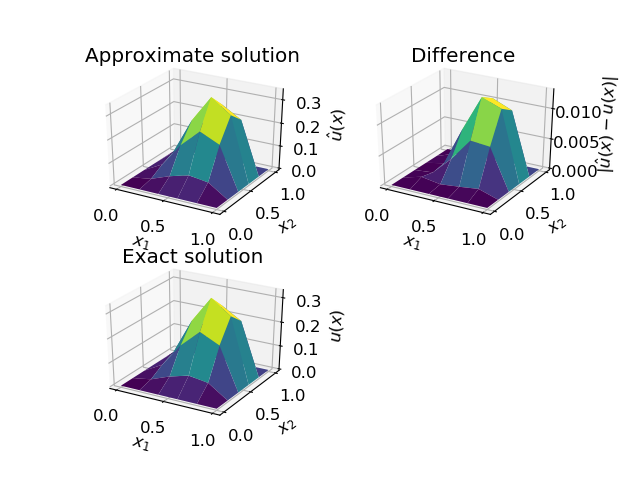
\includegraphics[width=0.75\textwidth]{Grafiken/3D_n=5}
    \vspace{-0.2cm}
    \captionof{figure}{Approximierte Lösung, exakte Lösung und deren absolute Differenz für $n = 5$}
    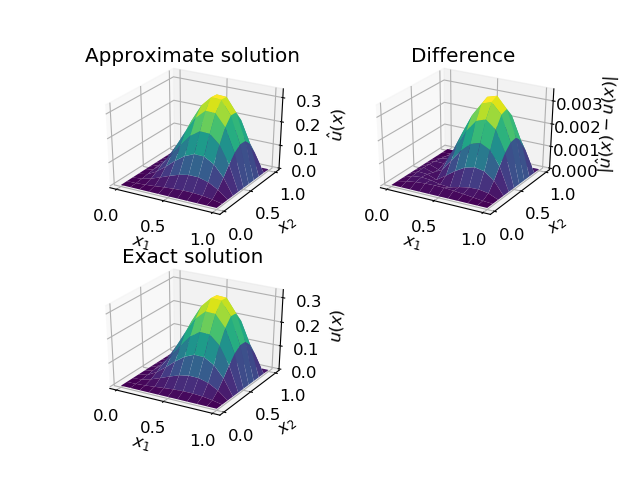
\includegraphics[width=0.75\textwidth]{Grafiken/3D_n=10}
    \vspace{-0.2cm}
    \captionof{figure}{Approximierte Lösung, exakte Lösung und deren absolute Differenz für $n = 10$}
    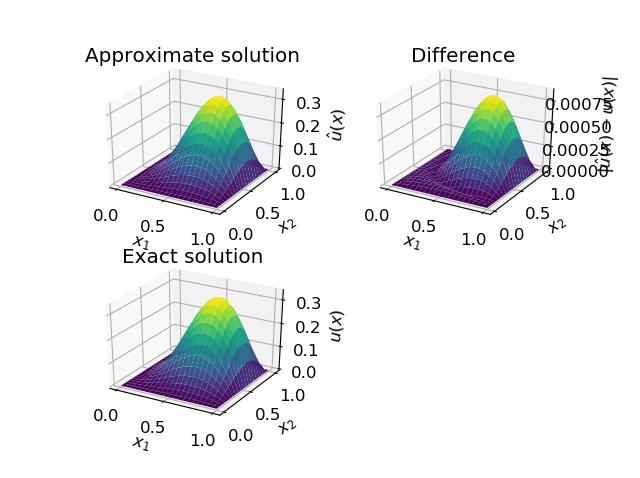
\includegraphics[width=0.75\textwidth]{Grafiken/3D_n=20}
    \vspace{-0.2cm}
    \captionof{figure}{Approximierte Lösung, exakte Lösung und deren absolute Differenz für $n = 20$}
}
\vspace{0.5cm}

Schon bei der sehr groben Diskretisierung mit $n=5$ kann man den Unterschied zwischen den beiden Lösungen mit bloßem Auge kaum erkennen, weshalb wir uns entschieden haben, auch die absolute Differenz der beiden darzustellen.
Wie man dort sehen kann, erreicht man durch Erhöhung der Anzahl der Intervalle eine immer genauere Approximation der exakten Lösungsfunktion. Die absolute Differenz der Approximation und der exakten Lösung hält sich in einer immer kleineren Größenordnung auf.

{
  \centering
    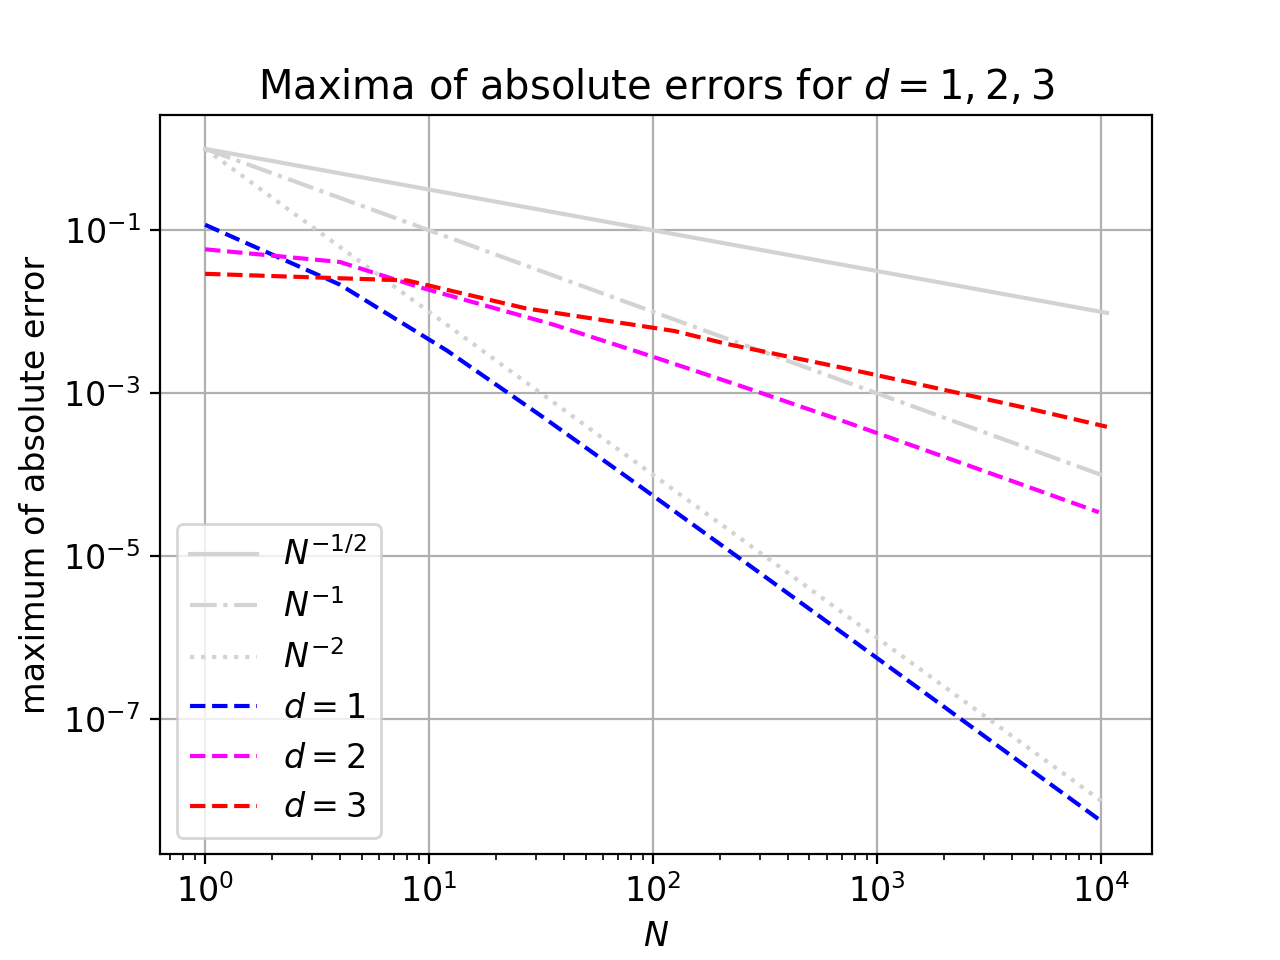
\includegraphics[width=0.75\textwidth]{Grafiken/loglogerr_d123_neu}
    \vspace{-0.2cm}
    \captionof{figure}{Konvergenzplot der maximalen absoluten Fehler in Abhängigkeit von $N$}
}
\vspace{0.5cm}

Man kann erkennen, dass mit größerem $N$, d.h. mit mehr Diskretisierungspunkten, der Fehler immer kleiner wird, wobei er sich bei höheren Dimensionen langsamer verkleinert.
Für $d=1$ lässt sich in der Abbildung eine quadratische Konvergenzgeschwindigkeit erkennen. Für $d=2$ hingegen nur noch eine lineare und bei $d=3$ nicht mal mehr eine lineare Konvergenzgeschwindigkeit. Dies lässt sich unter anderem zurückführen auf die Konvergenzgeschwindigkeit der zweiten finiten Differenz, die wir im ersten Bericht beschrieben haben.


\subsection{Rundungsfehler}
Für ein mathematisches Problem gibt seine Kondition den Faktor an, um den sich ein Fehler in den Eingangsdaten maximal auf die Lösung auswirken kann.
Die Kondition eines linearen Gleichungssystems $Ax = b$ mit regulärem $A\in\mathbb{R}^{N \times N}$ ist gegeben durch
\[cond(A) = ||A||\cdot||A^{-1}||\]\cite{tischendorf2019}

Die folgende Grafik zeigt die Entwicklung der Kondition der Matrix $A^{(d)}\in\mathbb{R}^{N \times N}$ in Abhängigkeit von $N$.

{
  \centering
    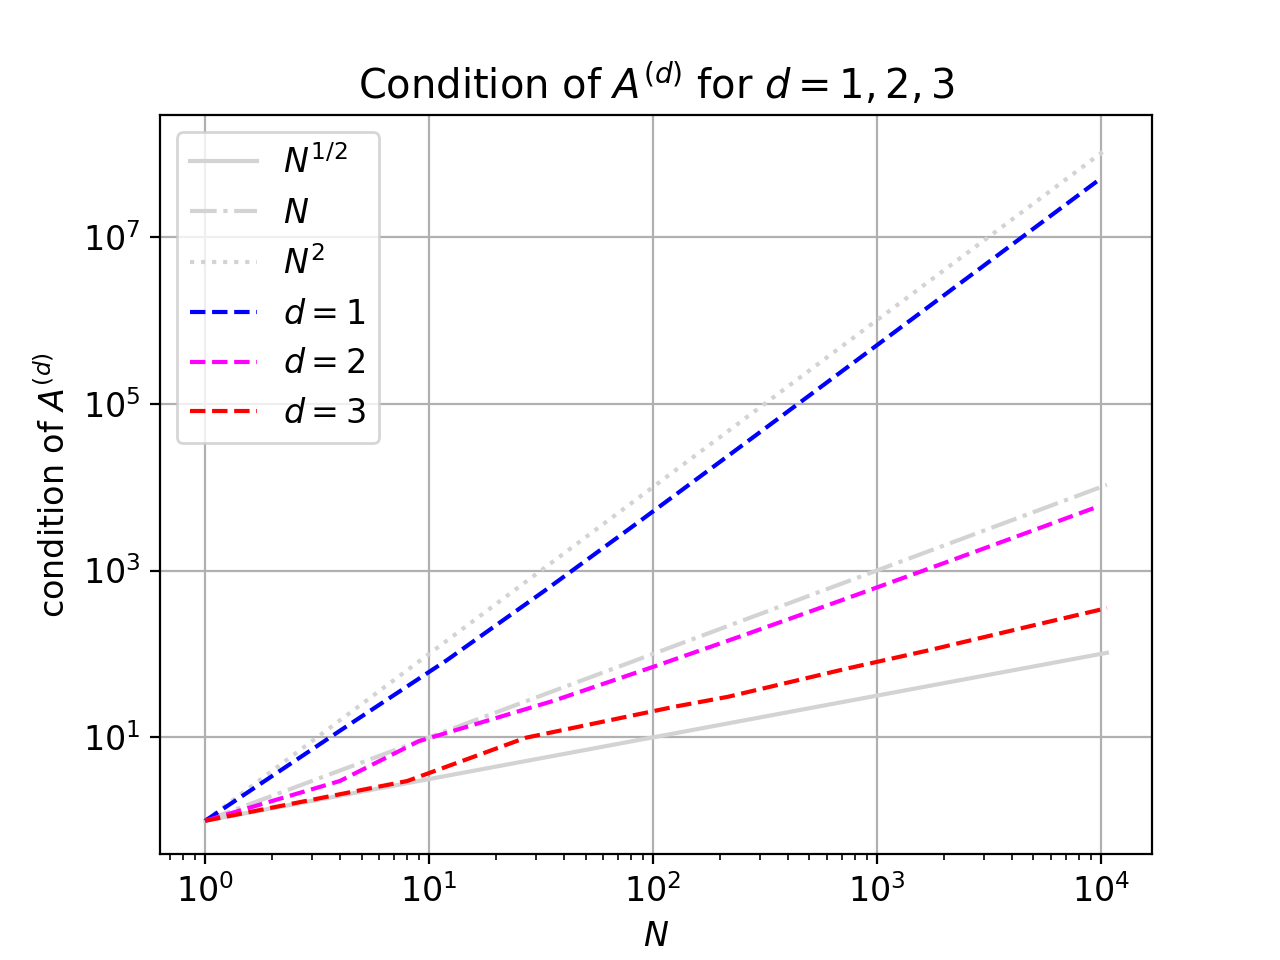
\includegraphics[width=0.75\textwidth]{Grafiken/loglogcond_d123_neu}
    \vspace{-0.2cm}
    \captionof{figure}{Kondition der Matrix in Abhängigkeit von $N$}
}
\vspace{0.5cm}

Man kann beobachten, dass die Kondition mit der gleichen Geschwindigkeit steigt, mit der für das jeweilige $d \in \{ 1, 2, 3\}$ der absolute Fehler sinkt.
Aufgrund der zunehmenden Größe/Dimension und Regularität von $A^{(d)}$ steigt auch die Kondition mit größer werdenden $N$.
Dass der gesamte Fehler trotzdem sinkt, weist darauf hin, dass sich die Rundungsfehler nicht sehr stark auf das Endergebnis auswirken.

Vergleicht man, wie in den Tabellen 1 bis 3 dargestelllt, die Kondition der Matrix $A^{(d)}$ mit der der Hilbertmatrix $H_N$ der gleichen Dimension, definiert durch

\[H_N =
\begin{pmatrix}
  1 & \frac{1}{2} & \frac{1}{3} & \cdots & \frac{1}{N} \\
  \frac{1}{2} & \frac{1}{3} & \frac{1}{4} & \cdots & \frac{1}{N+1} \\
  \frac{1}{3} & \frac{1}{4} & \frac{1}{5} & \cdots & \frac{1}{N+2} \\
  \vdots & \vdots & \vdots & \ddots & \vdots \\
  \frac{1}{N} & \frac{1}{N+1} & \frac{1}{N+2} & \cdots & \frac{1}{2N-1}
\end{pmatrix}\]\cite{tischendorf2019}

kann man erkennen, dass die Kondition der Matrix $A^{(d)}$ im Vergleich zur Hilbertmatrix nur ein sehr moderates Wachstum besitzt.

\begin{table}[ht!]
\centering
\begin{tabular}{|r|r|r|}
\hline
\textbf{N} & $\mathbf{cond(A^{(1)})}$ & $\mathbf{cond(H_N)}$   \\ \hline
1          & 1.0                       & 1.0                \\ \hline
2          & 3.0                       & 27.0               \\ \hline
3          & 8.0                       & 748.0              \\ \hline
4          & 12.0                      & 28375.0            \\ \hline
5          & 18.0                      & 943656.0          \\ \hline
6          & 24.0                      & 29070279.0         \\ \hline
7          & 32.0                      & 985194889.7        \\ \hline
8          & 40.0                      & 33872790819.5      \\ \hline
9          & 50.0                      & 1099650991701.1    \\ \hline
\end{tabular}
\caption{Vergleich der Kondition von $A^{(1)}$ und der entsprechenden Hilbertmatrix}
\end{table}

\begin{table}[ht!]
\centering
\begin{tabular}{|r|r|r|}
\hline
\textbf{N} & $\mathbf{cond(A^{(2)})}$  & $\mathbf{cond(H_N)}$       \\ \hline
1          & 1.0                       & 1.0                    \\ \hline
4          & 3.0                       & 28375.0                \\ \hline
9          & 9.0                       & 1099650991701.1        \\ \hline
16         & 13.3                      & 2.3e+18             \\ \hline
25         & 20.8                      & 1.7e+19 \\ \hline
36         & 27.4                      & 1.4e+19  \\ \hline
49         & 37.3                      & 3.8e+19  \\ \hline
64         & 46.3                      & 1.6e+19 \\ \hline
81         & 58.5                      & 8.0e+19  \\ \hline
\end{tabular}
\caption{Vergleich der Kondition von $A^{(2)}$ und der entsprechenden Hilbertmatrix}
\end{table}


\begin{table}[ht!]
\centering
\begin{tabular}{|r|r|r|}
\hline
\textbf{N} & $\mathbf{cond(A^{(3)})}$ & $\mathbf{cond(H_N)}$       \\ \hline
1          & 1.0                       & 1.0                    \\ \hline
8          & 3.0                       & 33872790819.5      \\ \hline
27         & 9.9                       & 1.6e+19 \\ \hline
64         & 14.5                      & 1.6e+19 \\ \hline
125        & 23.3                      & 5.9e+19  \\ \hline
216        & 30.6                      & 10.0e+20   \\ \hline
343        & 42.2                      & 10.0e+20  \\ \hline
512        & 52.2                      & 2.7e+22   \\ \hline
\end{tabular}
\caption{Vergleich der Kondition von $A^{(3)}$ und der entsprechenden Hilbertmatrix}
\end{table}

\pagebreak
\section{Untersuchungen zum Speicherplatz}
Für die Durchführung der Experimente haben wir die Matrizen wie schon im vorherigen Bericht beschrieben im \textit{sparse}-Format gespeichert.
Für die Matrizen $A^{(d)}$ hatten wir dort bereits ermittelt, dass sich dies schon für niedrige $n$ lohnt, da sich das \textit{sparse}-Format nur die nicht-Null-Einträge merkt.
Da für jeden nicht-Null-Eintrag drei Werte gespeichert werden müssen, lohnt es sich, das \textit{sparse}-Format zu nutzen, sobald weniger als ein Drittel der Einträge einer Matrix ungleich Null ist.
In der unteren Grafik sieht man die Anzahl der nicht-Null-Einträge von $A^{(d)}$ und der zugehörigen LU-Zerlegung für $d\in\{1, 2, 3\}$ in Abhängigkeit von $N$.
Desweiteren haben wir eine Linie eingezeichnet, die ein Drittel der Matrix Einträge repräsentiert.

{
  \centering
    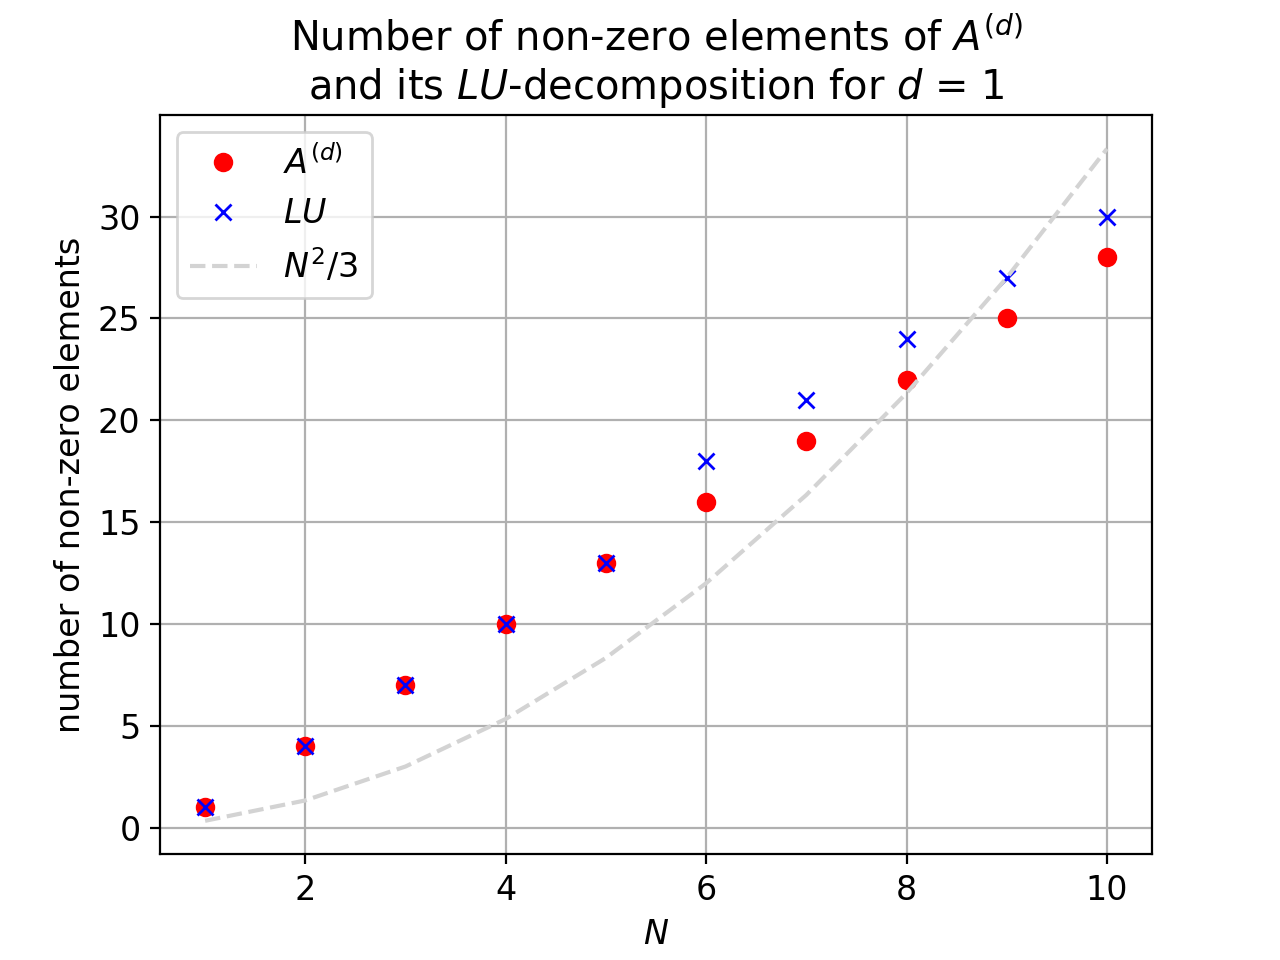
\includegraphics[width=0.75\textwidth]{Grafiken/non-zero_d1}
    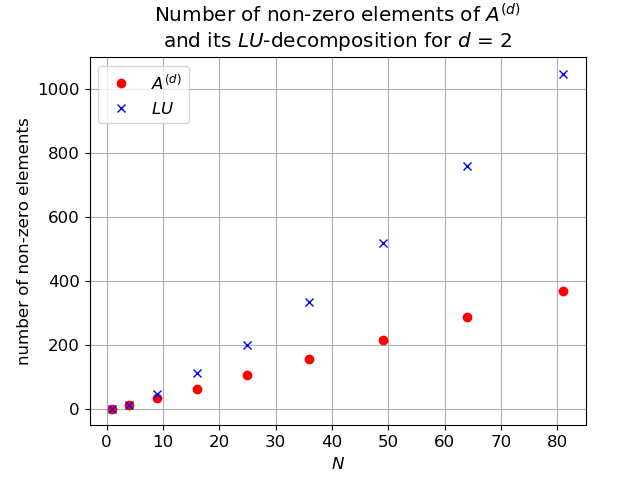
\includegraphics[width=0.75\textwidth]{Grafiken/non-zero_d2}
    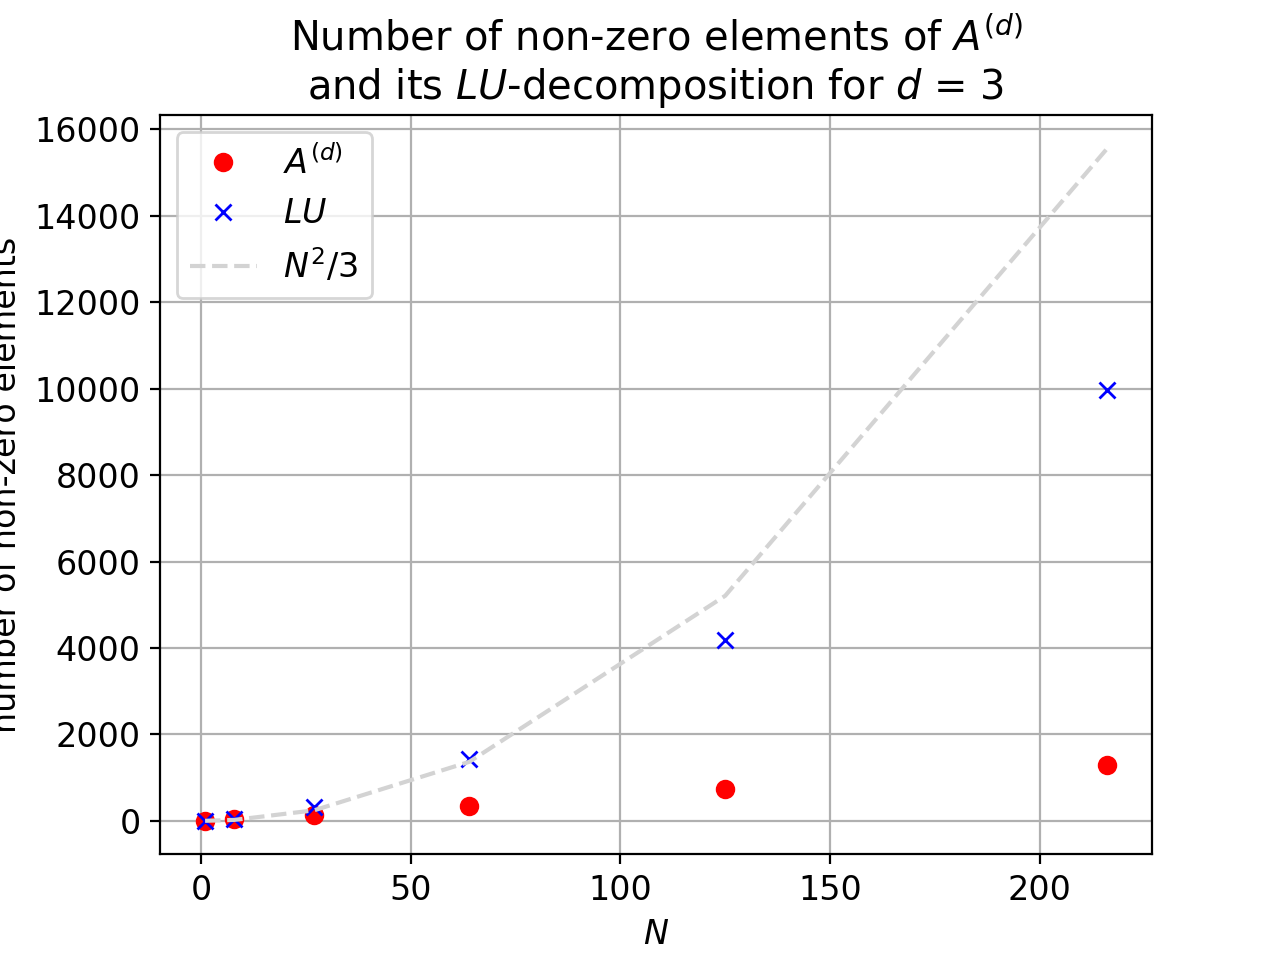
\includegraphics[width=0.75\textwidth]{Grafiken/non-zero_d3}
    \vspace{-0.2cm}
    \captionof{figure}{Anzahl der nicht-Null-Einträge von $A^{(d)}$ und der LU-Zerlegung für $d\in\{1, 2, 3\}$}
}
\vspace{0.5cm}

Für $d=1$ kann man beobachten, dass nach $N=9$ bzw. $n=10$  weniger als ein Drittel der Matrixeinträge von sowohl $A^{(d)}$ als auch der LU-Zerlegung ungleich Null ist.
Für $d=2$ gilt dies schon ab $N=25$ bzw. $n=6$ und für $d=3$ ab $N = 125$ bzw. auch für $n=6$.
Auch für die LU-Zerlegung lohnt es sich also schon für sehr niedrige $n$, die Matrix im \textit{sparse}-Format zu speichern.

\section{Zusammenfassung und Ausblick}
Im Rahmen dieser Arbeit haben wir für eine Beispielfunktion das Poisson-Problem mittels des direkten Verfahrens des Gauß-Algorithmus mit LU-Zerlegung für verschiedene Schrittweiten und Dimensionen gelöst.
Dabei haben wir beobachtet, dass für kleinere Schrittweiten zwar die Kondition der Matrix $A^{(d)}$ steigt, der Gesamtfehler jedoch immer kleiner wird und man eine ausreichend genaue Approximation der Lösung erreichen kann.
Wir haben desweiteren beobachtet, dass die Kondition der Matrix $A^{(d)}$ ein bedeutend langsameres Wachstum besitzt als die der Hilbertmatrix.
Zuletzt haben wir außerdem Untersuchungen zur Speichernutzung unternommen und festgestellt, dass aufgrund der vielen Null-Einträge der genutzten Matrizen die Nutzung des \textit{sparse}-Formates schon bei kleinen Intervallanzahlen lohnenswert ist.
Im nächsten Bericht werden wir weitere Verfahren untersuchen, die iterative Methoden nutzen, um das lineare Gleichungssystem zu lösen, und betrachten, wie sich diese Verfahren auf die Effizienz und Genauigkeit der Approximation auswirken.

\pagebreak

\bibliographystyle{plain}
\bibliography{serie3_literatur}

\appendix

\pagebreak

\section{Bedienung des Experimentierskriptes}

Es folgt eine kurze Anleitung zur Durchführung unserer Experimente über das angefügte Modul \texttt{main.py}.

\subsection{Lösen des Poisson-Problems}

Die approximierte Lösung \texttt{hat\_u} des Poisson-Problems für eine gegebene callable Funktion \texttt{f}, eine Dimension \texttt{d} und eine Intervallanzahl \texttt{n} ermittelt man mit den folgenden Aufrufen:

\begin{minted}{python}
  A = block_matrix.BlockMatrix(d, n)
  b = rhs.rhs(d, n, f)
  lu = A.get_lu()
  hat_u = linear_solvers.solve_lu(lu[0], lu[1], lu[2], lu[3], b)
\end{minted}

\subsection{Lösungsplot für Beispielfunktion mit d = 2}

Um die 3D-Plots der approximierten Lösungsfunktion, der exakten Lösungsfunktion und deren Differenz für eine bestimmte Schrittweite auszugeben, nutzen wir die Funktion \texttt{rhs.plot\_functions(u, f, n)}.
Hierbei ist \texttt{u} eine callable Funktion, die der exakten Lösung des Poisson-Problems entspricht, \texttt{f2} ist eine callable Funktion, für die das Problem gelöst werden soll und \texttt{n} ist die Anzahl der Intervalle.
Die in diesem Bericht genutzen Funktionen sind im Modul \texttt{main.py} vorgegeben als \texttt{u2} und \texttt{f2}.

\begin{minted}{python}
  def f2(x):
      """Function f of the Poisson-problem for d = 2
      """
      return (-2*np.pi*(x[1]*np.cos(np.pi*x[0])*np.sin(np.pi*x[1])+
                        x[0]*np.sin(np.pi*x[0])
                        *(np.cos(np.pi*x[1])- np.pi*x[1]*np.sin(np.pi*x[1]))))

  def u2(x):
      """Function u of the Poisson-problem for d = 2
      """
      return x[0]*np.sin(np.pi*x[0])*x[1]*np.sin(np.pi*x[1])

  def main():
  ## Lösungsplot für Bsp.funktion mit d = 2 für n = 5, 10, 20
      rhs.plot_functions(u2, f2, 5)
      rhs.plot_functions(u2, f2, 10)
      rhs.plot_functions(u2, f2, 20)
\end{minted}

\subsection{Fehler-/Konvergenzplots}

Unser Modul bietet Funktionalitäten, um die Fehlerplots entweder in separaten Plots für eine Dimension oder alle drei Dimensionen in einem Plot anzeigen zu lassen.
Um sie in separaten Plots anzuzeigen, nutzt man die Funktion \texttt{rhs.plot\_error(u, f, d, n\_list)}.
\texttt{u} und \texttt{f} sind hierbei wieder wie oben die Funktionen des Poisson-Problems als callables, \texttt{d} ist die Dimension als Integer und \texttt{n\_list} eine Liste von Intervallanzahlen, für die der Fehler ausgewertet werden soll.

\begin{minted}{python}
  ## Fehler-/Konvergenzplot für d = 1, 2, 3 in getrennten Grafiken

      rhs.plot_error(u1, f1, 1, np.geomspace(2, 10000, num=10, dtype=int))
      rhs.plot_error(u2, f2, 2, np.geomspace(2, 100, num=10, dtype=int))
      rhs.plot_error(u3, f3, 3, np.geomspace(2, 24, num=10, dtype=int))
\end{minted}

Die Funktion \texttt{rhs.plot\_error\_list(u\_list, f\_list, n\_list\_list)}, der man Listen von Funktionen u und f übergibt, in aufsteigender Reihenfolge der Dimensionen 1 bis 3 und eine Liste von Listen an Intervallanzahlen für die Dimensionen 1 bis 3, zeigt alle Fehlerplots in einer Grafik an.

\begin{minted}{python}
  ## Fehler-/Konvergenzplot für d = 1, 2, 3 in einer Grafik

      n_list = [np.geomspace(2, 10000, num=10, dtype=int),
                np.geomspace(2, 100, num=10, dtype=int),
                np.geomspace(2, 24, num=10, dtype=int)]
      rhs.plot_error_list([u1, u2, u3], [f1, f2, f3], n_list)
\end{minted}

\subsection{Konditionsplot}

Um die Konditionen der Matrizen $A^{(d)}$ plotten zu lassen, nutzt man die Funktion \\\texttt{block\_matrix.plot\_cond\_list(n\_list\_list}, wobei \texttt{n\_list\_list} wieder eine Liste von Listen an Intervallanzahlen für die Dimensionen 1 bis 3 ist.

\begin{minted}{python}
  ## Konditionsplot von A^(d) für d = 1, 2, 3 in einer Grafik

      n_list = [np.geomspace(2, 10000, num=10, dtype=int),
                np.geomspace(2, 100, num=10, dtype=int),
                np.geomspace(2, 24, num=10, dtype=int)]
      block_matrix.plot_cond_list(n_list)
\end{minted}

\subsection{Vergleich mit Kondition der Hilbertmatrix}

Mit der Funktion \texttt{block\_matrix.print\_cond(n\_list, d)} kann man für die Intervallanzahlen in \texttt{n\_list} und die Dimension \texttt{d} die Konditionen von $A^{(d)}$ ausgeben lassen.
Die Funktion \texttt{print\_cond\_hilbert(n\_list, d)} macht dasselbe für die entsprechende Hilbertmatrix.
Alternativ könnte man sich die Kondition der Hilbertmatrix auch mit \\\texttt{plot\_cond\_hilbert(n\_list, d)} als Grafik ausgeben lassen.

\begin{minted}{python}
## Konditionsprint A^(d) und Hilbertmatrix von gleicher
## Dimension = (n-1)^d mit d = 1, 2, 3

    block_matrix.print_cond(range(2, 11), 1)
    print_cond_hilbert(range(2, 11), 1)

    block_matrix.print_cond(range(2, 11), 2)
    print_cond_hilbert(range(2, 11), 2)

    block_matrix.print_cond(range(2, 11), 3)
    print_cond_hilbert(range(2, 11), 3)
\end{minted}

\subsection{Untersuchung der Sparsity}

Um die Anzahl der nicht-Null-Einträge der Matrix $A^{(d)}$ und ihrer LU-Zerlegung für die drei Dimensionen plotten zu lassen, nutzt man die Funktion \\\texttt{block\_matrix.plot\_non\_zeros(n\_list)}, der man wieder eine Liste von Intervallanzahlen in \texttt{n\_list} übergibt.

\begin{minted}{python}
  ## Sparsity von A^(d) und ihrer LU-Zerlegung für
  ## d = 1, 2, 3 in getrennten Grafiken

      block_matrix.plot_non_zeros(range(2, 8))
\end{minted}

\end{document}